%%%%%%%%%%%%%%%%%%%%%%%%%%%%%%%%%%%%%%%%%
% Beamer Presentation
% LaTeX Template
% Version 1.0 (10/11/12)
%
% This template has been downloaded from:
% http://www.LaTeXTemplates.com
%
% License:
% CC BY-NC-SA 3.0 (http://creativecommons.org/licenses/by-nc-sa/3.0/)
%
%%%%%%%%%%%%%%%%%%%%%%%%%%%%%%%%%%%%%%%%%

%----------------------------------------------------------------------------------------
%	PACKAGES AND THEMES
%----------------------------------------------------------------------------------------

\documentclass{beamer}

\mode<presentation> {

% The Beamer class comes with a number of default slide themes
% which change the colors and layouts of slides. Below this is a list
% of all the themes, uncomment each in turn to see what they look like.

%\usetheme{default}
%\usetheme{AnnArbor}
%\usetheme{Antibes}
%\usetheme{Bergen}
%\usetheme{Berkeley}
%\usetheme{Berlin}
%\usetheme{Boadilla}
%\usetheme{CambridgeUS}
%\usetheme{Copenhagen}
%\usetheme{Darmstadt}
%\usetheme{Dresden}
%\usetheme{Frankfurt}
%\usetheme{Goettingen}
%\usetheme{Hannover}
%\usetheme{Ilmenau}
%\usetheme{JuanLesPins}
%\usetheme{Luebeck}
\usetheme{Madrid}
%\usetheme{Malmoe}
%\usetheme{Marburg}
%\usetheme{Montpellier}
%\usetheme{PaloAlto}
%\usetheme{Pittsburgh}
%\usetheme{Rochester}
%\usetheme{Singapore}
%\usetheme{Szeged}
%\usetheme{Warsaw}

% As well as themes, the Beamer class has a number of color themes
% for any slide theme. Uncomment each of these in turn to see how it
% changes the colors of your current slide theme.

%\usecolortheme{albatross}
%\usecolortheme{beaver}
%\usecolortheme{beetle}
%\usecolortheme{crane}
%\usecolortheme{dolphin}
%\usecolortheme{dove}
%\usecolortheme{fly}
%\usecolortheme{lily}
%\usecolortheme{orchid}
%\usecolortheme{rose}
%\usecolortheme{seagull}
%\usecolortheme{seahorse}
%\usecolortheme{whale}
%\usecolortheme{wolverine}

%\setbeamertemplate{footline} % To remove the footer line in all slides uncomment this line
%\setbeamertemplate{footline}[page number] % To replace the footer line in all slides with a simple slide count uncomment this line

%\setbeamertemplate{navigation symbols}{} % To remove the navigation symbols from the bottom of all slides uncomment this line
}

\usepackage{graphicx} % Allows including images
\usepackage{booktabs} % Allows the use of \toprule, \midrule and \bottomrule in tables
\usepackage{multirow}
\usepackage{multicol}
\usepackage{adjustbox}
\usepackage{array}
\usepackage{tikz}
\usepackage{soul}
\usetikzlibrary{shapes.geometric, arrows, positioning, fit}
\usepackage[latin1]{inputenc}
\newcommand{\xmark}{\textcolor{red}{\text{\sffamily X}}}
\newcommand{\cmark}{\textcolor{green}{\checkmark}}
\newcommand{\tr}{\text{tr}}
\newcommand{\E}{\textbf{E}}
\newcommand{\diag}{\text{diag}}
\newcommand{\argmax}{\text{argmax}}
\newcommand{\argmin}{\text{argmin}}
\newcommand{\Cov}{\text{Cov}}
\newcommand{\Var}{\text{Var}}
\newcommand{\Vol}{\text{Vol}}
\newcommand{\bx}{\boldsymbol{x}}
\newcommand{\by}{\boldsymbol{y}}
\newcommand{\bX}{\boldsymbol{X}}
\newcommand{\bY}{\boldsymbol{Y}}
\sethlcolor{gray}
\makeatletter
\newcommand\SoulColor{%
  \let\set@color\beamerorig@set@color
  \let\reset@color\beamerorig@reset@color}
\makeatother
\definecolor{color1}{RGB}{128,13,13}
\definecolor{color2}{RGB}{70,128,13}
\definecolor{color3}{RGB}{13,128,128}
\definecolor{color4}{RGB}{70,13,128}

\newcommand{\faceA}{
\includegraphics[scale = 0.15]{face_photos/Amelia_Vega_0002.png}}
\newcommand{\faceB}{
\includegraphics[scale = 0.15]{face_photos/Jean-Pierre_Raffarin_0004.png}}
\newcommand{\faceC}{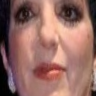
\includegraphics[scale = 0.15]{face_photos/Liza_Minnelli_0003.png}}
\newcommand{\faceD}{
\includegraphics[scale = 0.15]{face_photos/Patricia_Clarkson_0001.png}}

%tikz stufff


%----------------------------------------------------------------------------------------
%	TITLE PAGE
%----------------------------------------------------------------------------------------


%Extrapolating prediction error for 'extreme' multi-class classification

%with Rakesh Achanta and Yuval Benjamini

%'Extreme' classification refers to the classification with extremely
%large (on the order of millions) of labels, such as in photo or
%website annotation.  A natural question in these settings is whether
%the data is sufficiently rich to support high-accuracy classification
%with such a large label space.  Therefore, in this work, we address
%the question of predicting how well a classifier will scale with an
%increased number of classes, based on its performance in a smaller but
%representative classification problem. Under the assumption that the
%classes are sampled exchangeably, and under the assumption that the
%classifier is based on marginal probabilities (e.g. QDA or Naive
%Bayes), we derive a method for performance extrapolation based on
%unbiased estimation. We investigate the robustness of our methods to
%non-marginal classifiers in simulations and one optical character
%recognition example.


% Image sources
% http://sociable.co/social-media/how-to-disable-facebook-facial-recognition/
% https://alexanderskv.wordpress.com/2012/06/04/facial-recognition/
% https://medium.com/@ageitgey/machine-learning-is-fun-part-4-modern-face-recognition-with-deep-learning-c3cffc121d78#.fzgvan3ii

\title[Defense]{Supervised Evaluation of Representations}

\author{Charles Zheng} % Your name
\institute[Stanford] % Your institution as it will appear on the bottom of every slide, may be shorthand to save space
{Stanford University}
\date{\today} % Date, can be changed to a custom date

\begin{document}

\begin{frame}
\titlepage % Print the title page as the first slide
%(Joint work with Rakesh Achanta and Yuval Benjamini.)
\end{frame}

\section{Introduction}

%\begin{frame}
%\sectionpage
%\end{frame}

\begin{frame}
\frametitle{What is a representation?}
\begin{itemize}
\item It is often hypothesized that \emph{complex objects} (images, sounds, etc.) can be mapped into a \emph{low-dimensional} space
\item A \emph{representation} is a nonlinear, dimensionality-reducing mapping
\end{itemize}
\end{frame}

\begin{frame}
\frametitle{Why do we care?}
\begin{itemize}
\item Application 1: Neuroscience.  Different regions of the brain have different representations of the same sensory stimuli.
\item Application 2: Machine learning.  A good representation leads to more accurate prediction.
\end{itemize}
\end{frame}

\begin{frame}
\frametitle{Example: Facial recognition}
\begin{itemize}
\item Used to tag images in software, security \pause
\item Preprocessing
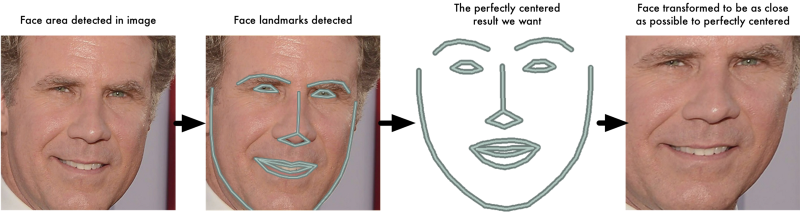
\includegraphics[scale = 0.4]{face_alignment.png}
\pause
\item Feature extraction
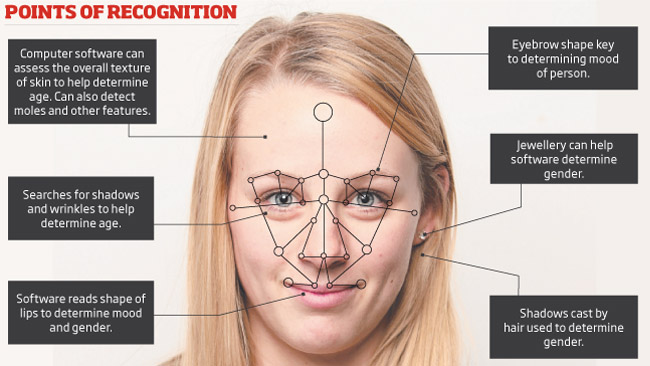
\includegraphics[scale = 0.4]{facerec_features.jpg}
\end{itemize}
\end{frame}

\begin{frame}
\frametitle{What defines a good representation?}

\end{frame}


\section{Randomized classification and extrapolation}

\begin{frame}
\sectionpage
\end{frame}

\begin{frame}
\frametitle{Multi-class classification}
\begin{columns}
\begin{column}{0.5\textwidth}
\begin{center}
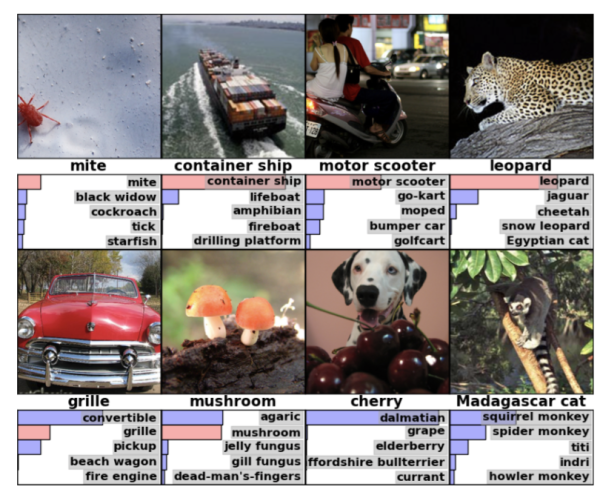
\includegraphics[scale = 0.4]{imagenet-fig4l.png}
\end{center}
\vspace{0.2in}
\tiny{from Krizhevsky et al. 2012}
\end{column}
\begin{column}{0.5\textwidth}
\begin{itemize}
\item MNIST digit recognition: 10 categories
\item Human motion database: 51 categories
\item ImageNet: 22,000 categories
\item Wikipedia: 325,000 categories
\end{itemize}
\end{column}
\end{columns}
\end{frame}



\begin{frame}
\frametitle{Accuracy vs. number of classes}
%Kay (2008) image identification task in functional MRI.
\begin{center}
%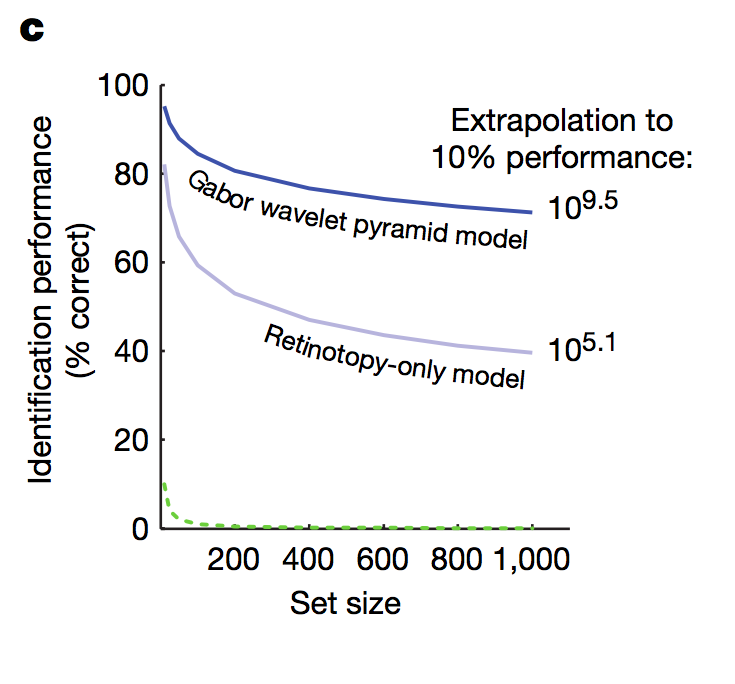
\includegraphics[scale = 0.2, clip=true, trim = 0 0in 0 0]{kay_extrapolation.png}
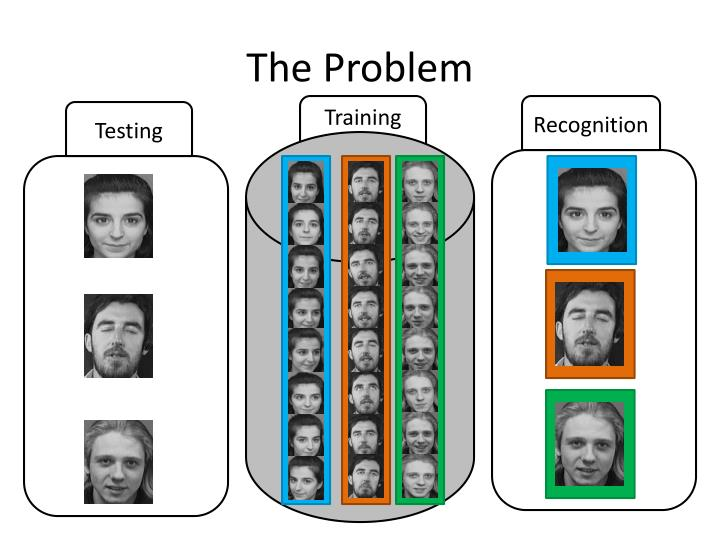
\includegraphics[scale = 0.2]{face_rec_the-problem-n.jpg}\pause
\hspace{0.2in}
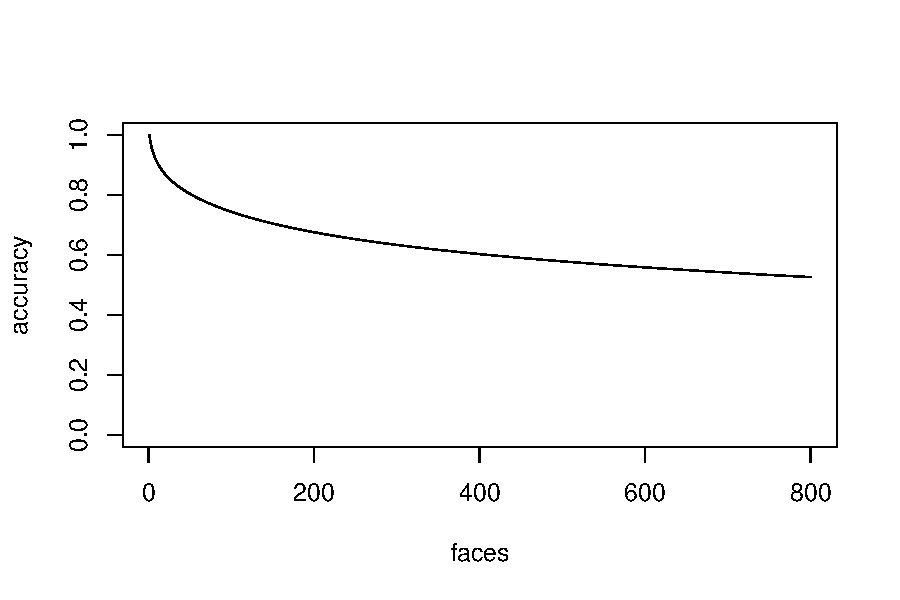
\includegraphics[scale = 0.3]{../facerec/acc_plot1.pdf}\pause
\end{center}

How does the accuracy scale with the number of classes (faces)?
\end{frame}




\begin{frame}
\frametitle{Setup}

\begin{center}
\begin{tabular}{c|c}
1. Population of categories $\pi(y)$ & 
2. Subsample $k$ labels, $y_1,\hdots, y_k$\\
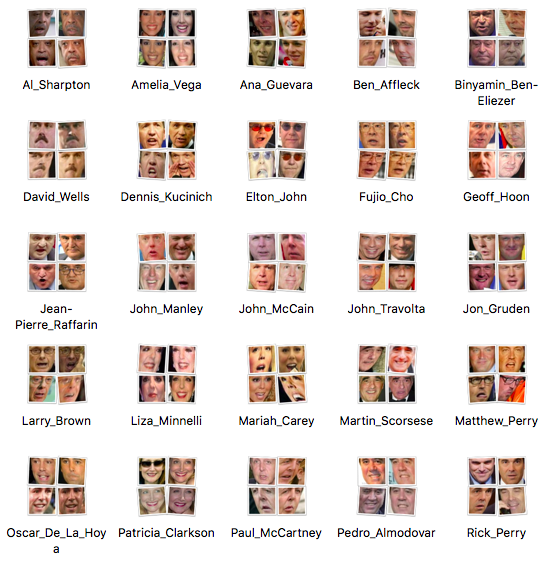
\includegraphics[scale = 0.2]{photo_folders.png} &
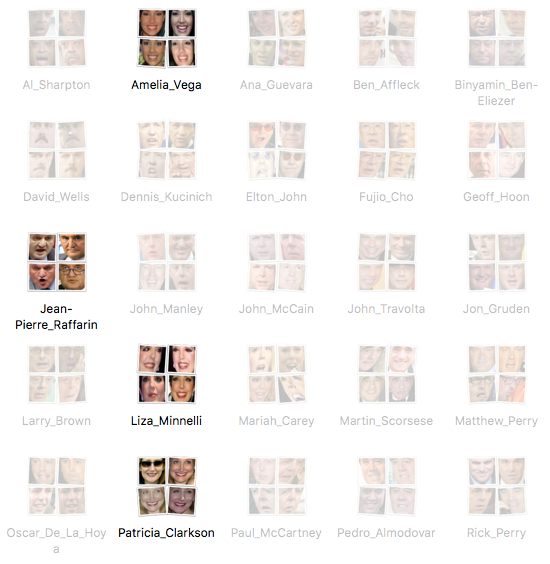
\includegraphics[scale = 0.2]{photo_folders2.png}
\end{tabular}
\end{center}

\end{frame}



\begin{frame}
\frametitle{Setup}

\vspace{0.1in}
3. Collect training and test data $x_j^{(i)}$ (faces) for labels (people) $\{y_1,\hdots, y_k\}$.

\begin{center}
\begin{tabular}{|c|ccc|c|}
\hline
Label & & Training & & Test\\ \hline
$y_1$=Amelia & 
  $x_1^{(1)} = $
\includegraphics[scale = 0.2]{face_photos/Amelia_Vega_0001.png} &  
  $x_1^{(2)} = $
\includegraphics[scale = 0.2]{face_photos/Amelia_Vega_0002.png} &  
  $x_1^{(3)} = $
\includegraphics[scale = 0.2]{face_photos/Amelia_Vega_0003.png} &  
  $x_1^{*} = $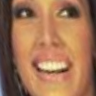
\includegraphics[scale = 0.2]{face_photos/Amelia_Vega_0004.png} \\ \hline
$y_2$=Jean-Pierre & 
  $x_2^{(1)} = $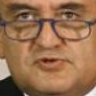
\includegraphics[scale = 0.2]{face_photos/Jean-Pierre_Raffarin_0001.png} &  
  $x_2^{(2)} = $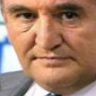
\includegraphics[scale = 0.2]{face_photos/Jean-Pierre_Raffarin_0002.png} &  
  $x_2^{(3)} = $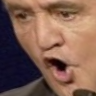
\includegraphics[scale = 0.2]{face_photos/Jean-Pierre_Raffarin_0003.png} &  
  $x_2^{*} = $
\includegraphics[scale = 0.2]{face_photos/Jean-Pierre_Raffarin_0004.png} \\ \hline
$y_3$=Liza & 
  $x_3^{(1)} = $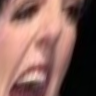
\includegraphics[scale = 0.2]{face_photos/Liza_Minnelli_0001.png} &  
  $x_3^{(2)} = $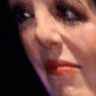
\includegraphics[scale = 0.2]{face_photos/Liza_Minnelli_0002.png} &  
  $x_3^{(3)} = $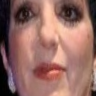
\includegraphics[scale = 0.2]{face_photos/Liza_Minnelli_0003.png} &  
  $x_3^{*} = $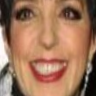
\includegraphics[scale = 0.2]{face_photos/Liza_Minnelli_0004.png} \\ \hline
$y_4$=Patricia & 
  $x_4^{(1)} = $
\includegraphics[scale = 0.2]{face_photos/Patricia_Clarkson_0001.png} &  
  $x_4^{(2)} = $
\includegraphics[scale = 0.2]{face_photos/Patricia_Clarkson_0002.png} &  
  $x_4^{(3)} = $
\includegraphics[scale = 0.2]{face_photos/Patricia_Clarkson_0003.png} &  
  $x_4^{*} = $
\includegraphics[scale = 0.2]{face_photos/Patricia_Clarkson_0004.png} \\ \hline
\end{tabular}
\end{center}


\vspace{0.1in}
4. Train a classifier and compute test error. \pause

\vspace{0.1in}
\textbf{Can we analyze how error depends on }$k$?
\end{frame}


\begin{frame}
\frametitle{Key assumption: marginal classifier}
\begin{itemize}
\item The classifier is \emph{marginal} if it learns a model \emph{independently} for each class.\pause
\item Examples: LDA/QDA 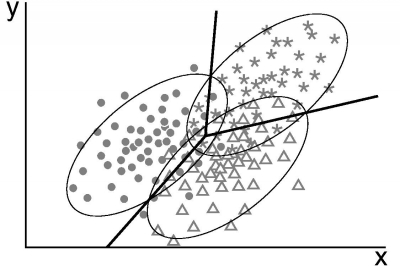
\includegraphics[scale = 0.2]{discriminant.jpg}, \pause
na\"{i}ve Bayes 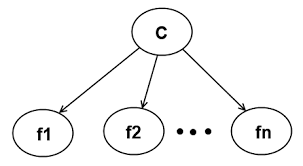
\includegraphics[scale = 0.2]{naive_bayes.png} \pause
\item Non-marginal classifiers: Multinomial logistic, multilayer neural networks, k-nearest neighbors
\end{itemize}
\end{frame}

\begin{frame}
\frametitle{Definitions}

$\hat{F}_{y^{(i)}}$ is the empirical distribution obtained from the training data for label $y^{(i)}$.

\begin{center}
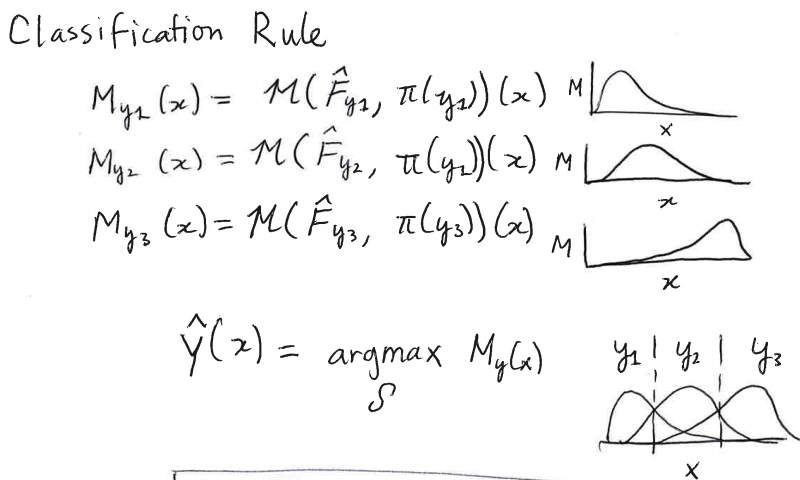
\includegraphics[scale = 0.2]{../info_theory_paper/extrapolation_figures/classification_rule.png}
\end{center}
\end{frame}

\begin{frame}

\begin{center}
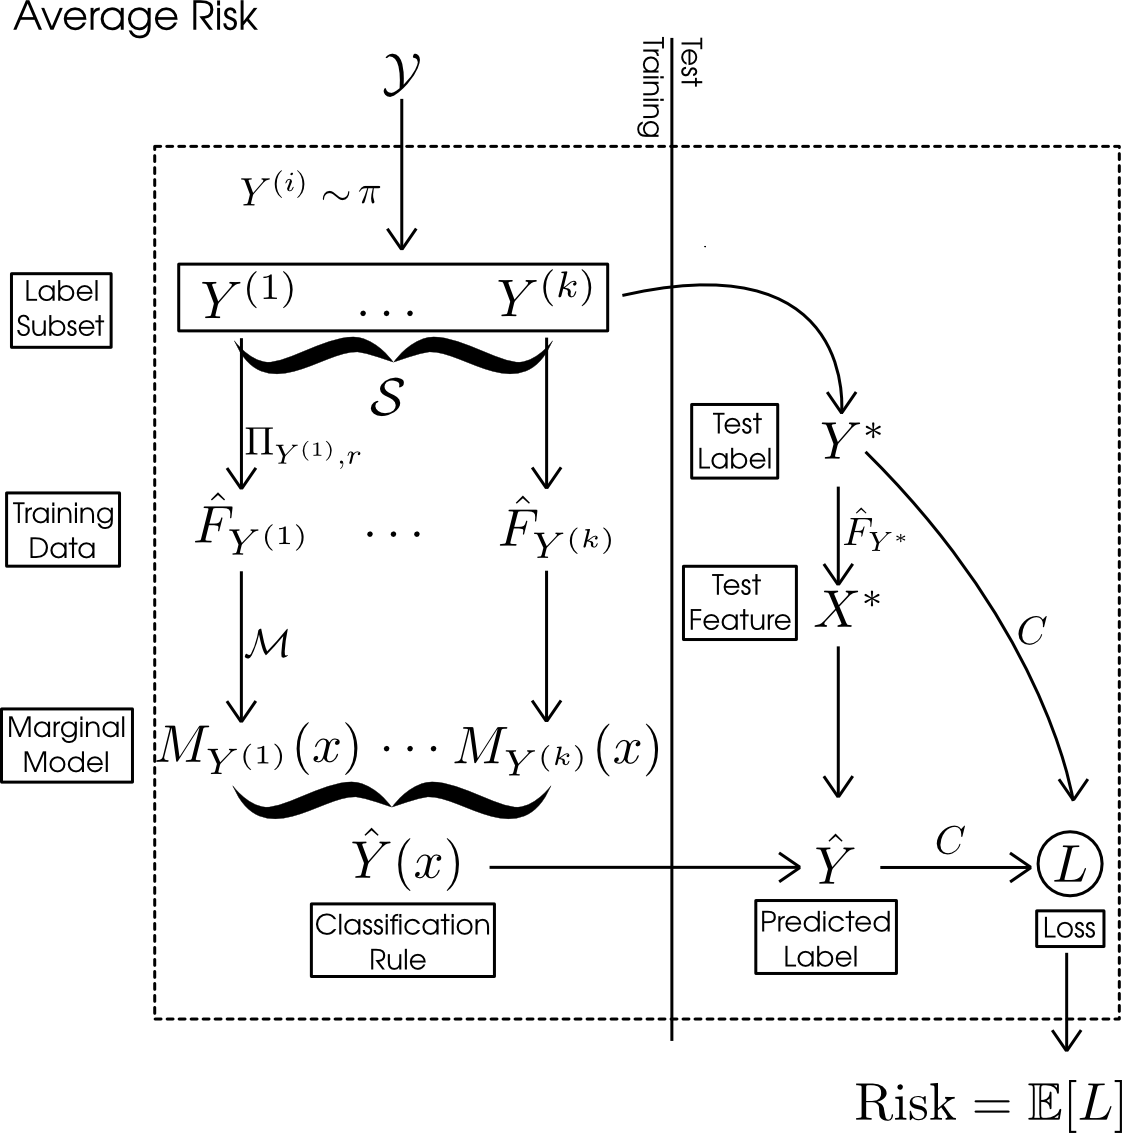
\includegraphics[scale = 0.2]{../info_theory_paper/extrapolation_figures/average_risk.png}
\end{center}
\end{frame}


\begin{frame}
\frametitle{Theoretical Result}

\textbf{Theorem. (Z.}, Achanta, Benjamini.)
Suppose $\pi$, $\{F_y\}_{y \in \mathcal{Y}}$ and marginal classifier
$\mathcal{F}$ satisfy \emph{(some regularity condition)}.  Then, 
there exists some function $\bar{D}(u)$ on $[0,1] \to [0,1]$ such that
the $k$-class average risk is given by
\[
\text{AvRisk}_k = (k-1) \int \bar{D}(u) u^{k-2} du.
\]
\pause

\vspace{1in}
What is this $\bar{D}(u)$ function? We will explain in the following toy example...
\end{frame}

\begin{frame}
\frametitle{Toy example}
$Y_1,\hdots, Y_k \stackrel{iid}{\sim} N(0, 1);$\pause

$X|Y \sim N(\rho Y, 1-\rho^2)$ i.e. $(Y, X) \sim N(0, \begin{pmatrix}1 & \rho\\\rho & 1\end{pmatrix}).$

\begin{center}
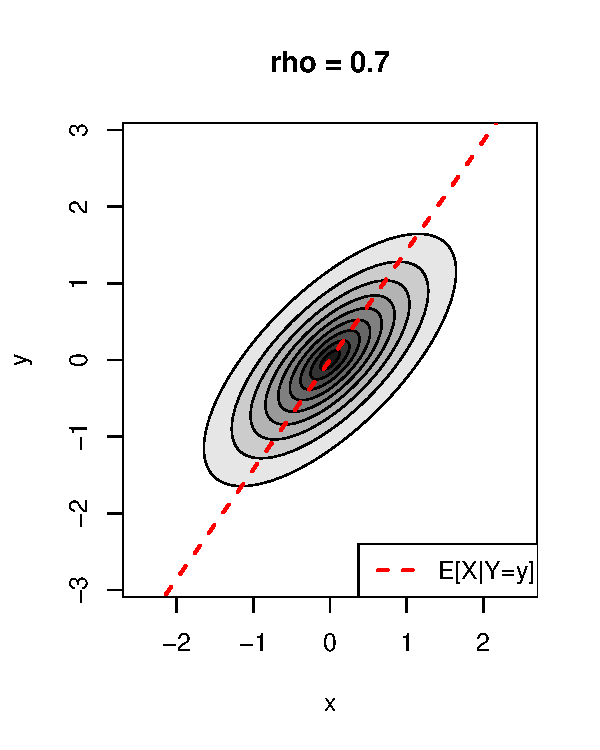
\includegraphics[scale = 0.5, clip = true, trim = 0 0 0 0.5in]{../extrapolation/illus_rho_0_7.pdf}
\end{center}

\end{frame}





\begin{frame}
\frametitle{Toy example}

\begin{center}
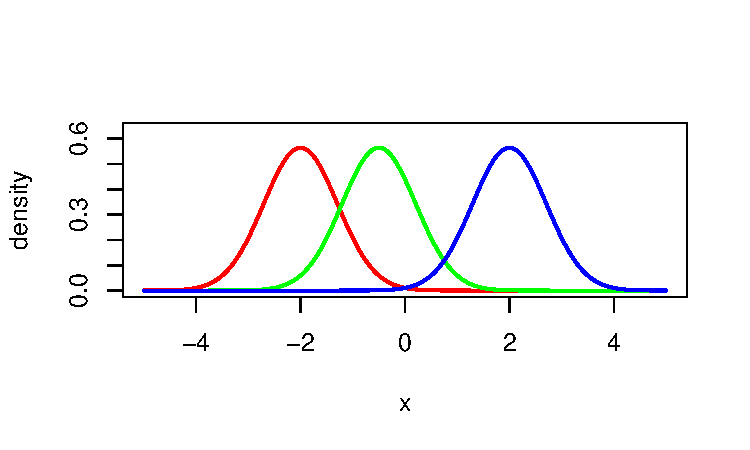
\includegraphics[scale = 0.5, clip = true, trim = 0 0.8in 0 0.8in]{../extrapolation/illus_example1a.pdf}
\end{center}

\begin{itemize}
\item Suppose $k=3$, and we draw $Y_1, Y_2, Y_3$.
\item The \emph{Bayes rule} is the optimal classifier and depends on knowing the true densities:
\[
\hat{y}(x) = \text{argmax}_{y_i} p(x|y_i)
\]
\item The \emph{Bayes Risk}, which is the misclassification rate of the optimal classifier.
\end{itemize}

\end{frame}

\begin{frame}
\frametitle{Toy example}

\begin{center}
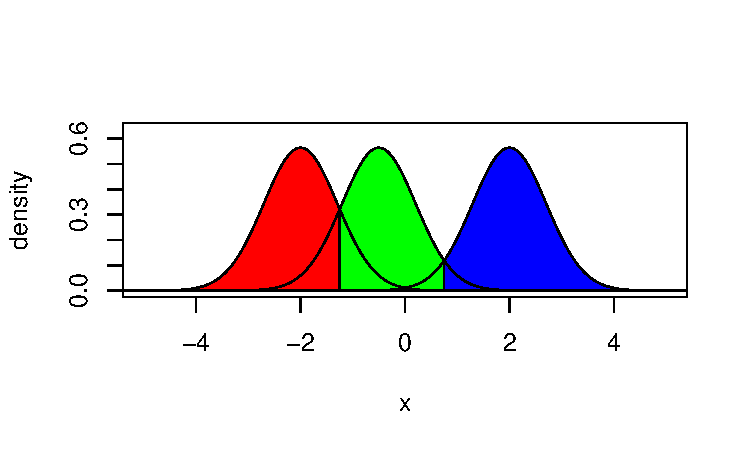
\includegraphics[scale = 0.5, clip = true, trim = 0 0 0 0.5in]{../extrapolation/illus_example1b.pdf}
\end{center}

\begin{itemize}
\item The \emph{Bayes Risk} is the expected test error of the Bayes rule,
\[
\frac{1}{k} \sum_{i=1}^k \Pr[\hat{y}(x) \neq Y| Y = y_i]
\]
\end{itemize}
% = 1 - \frac{1}{k}\int \max_{i=1}^k p(x|y_i) dx.

\end{frame}

\begin{frame}
\frametitle{Toy example}
\begin{columns}
\begin{column}{0.5\textwidth}
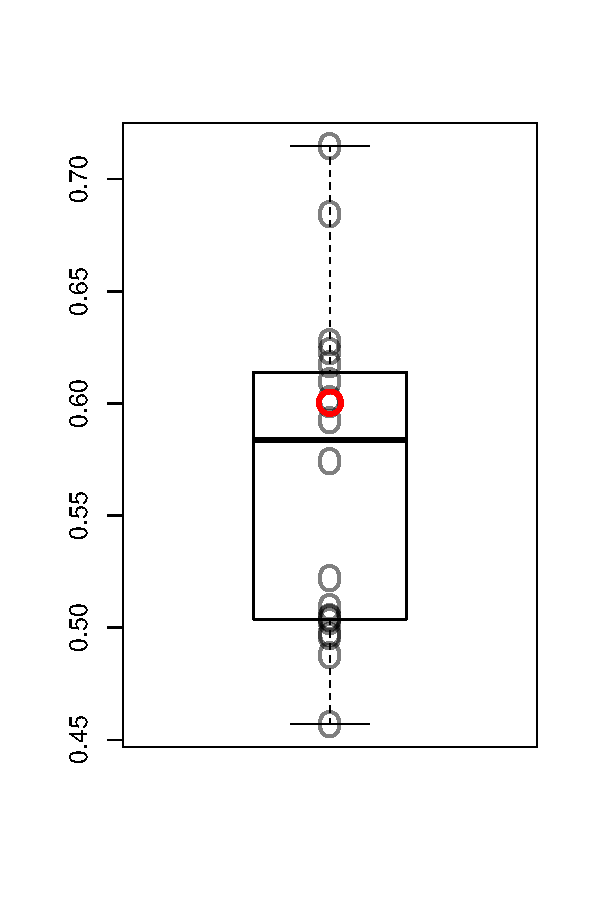
\includegraphics[scale = 0.5]{../extrapolation/autoplots/box4_1.pdf}
\end{column}
\begin{column}{0.5\textwidth}
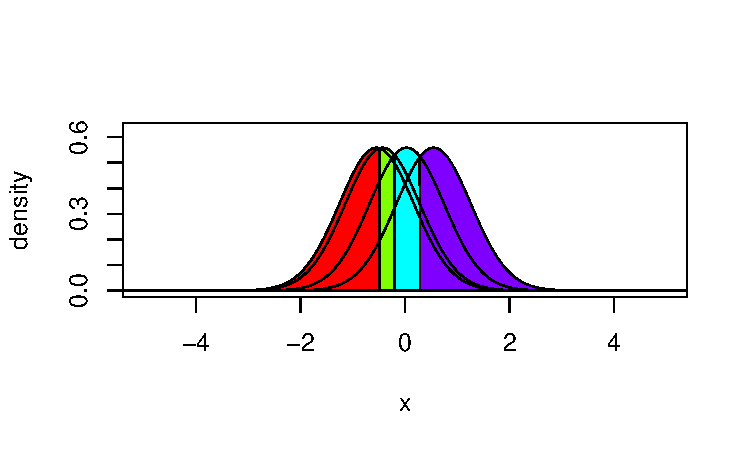
\includegraphics[scale = 0.5]{../extrapolation/autoplots/dens4_1.pdf}
\end{column}
\end{columns}
\end{frame}

\begin{frame}
\frametitle{Toy example}
\begin{columns}
\begin{column}{0.5\textwidth}
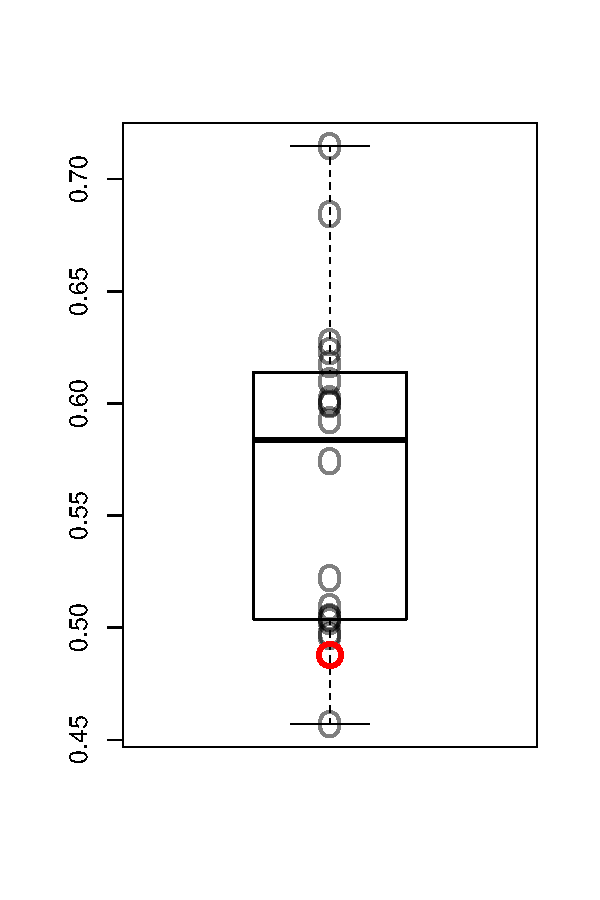
\includegraphics[scale = 0.5]{../extrapolation/autoplots/box4_2.pdf}
\end{column}
\begin{column}{0.5\textwidth}
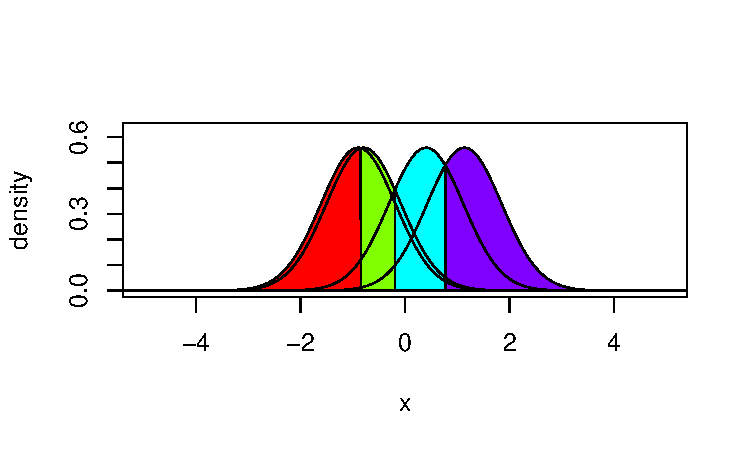
\includegraphics[scale = 0.5]{../extrapolation/autoplots/dens4_2.pdf}
\end{column}
\end{columns}
\end{frame}

\begin{frame}
\frametitle{Toy example}
\begin{columns}
\begin{column}{0.5\textwidth}
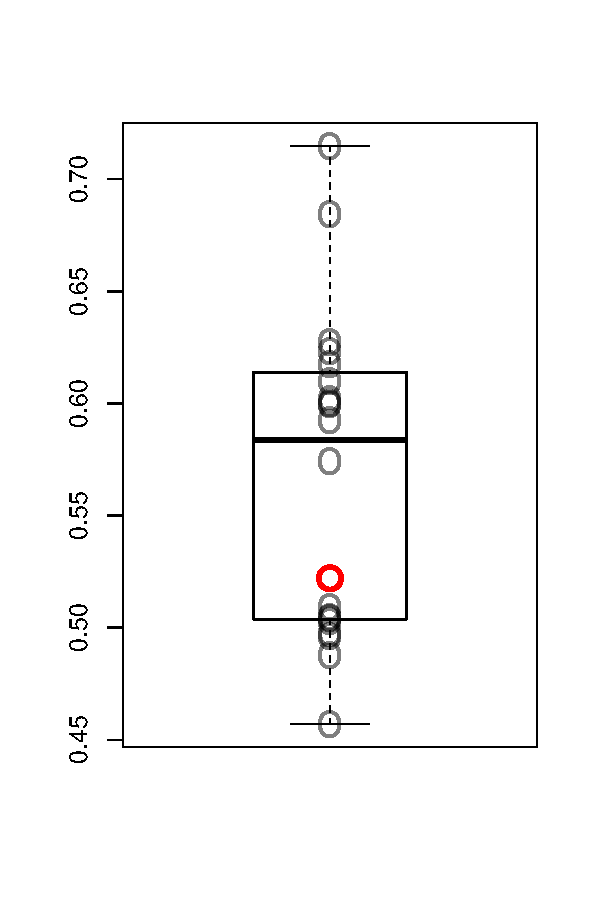
\includegraphics[scale = 0.5]{../extrapolation/autoplots/box4_3.pdf}
\end{column}
\begin{column}{0.5\textwidth}
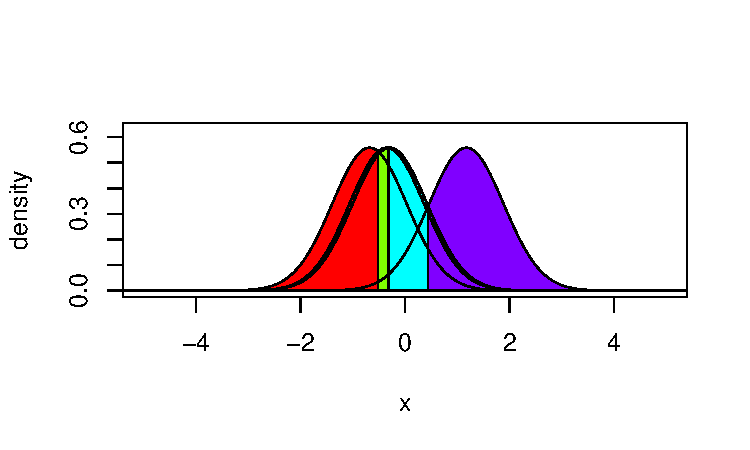
\includegraphics[scale = 0.5]{../extrapolation/autoplots/dens4_3.pdf}
\end{column}
\end{columns}
\end{frame}

\begin{frame}
\frametitle{Toy example}
\begin{center}
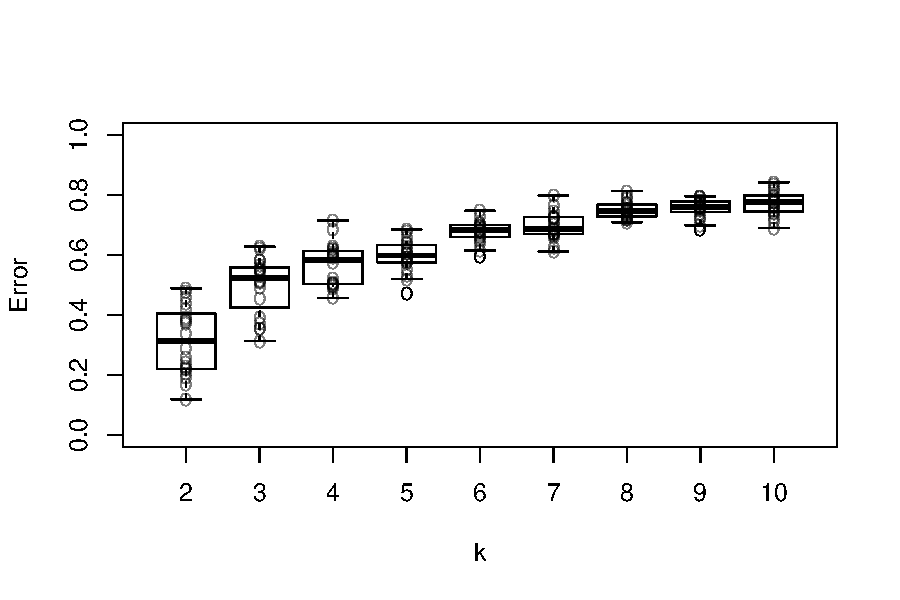
\includegraphics[scale = 0.5]{../extrapolation/autoplots/all_box.pdf}
\end{center}
\end{frame}

\begin{frame}
\frametitle{Toy example}
\begin{center}
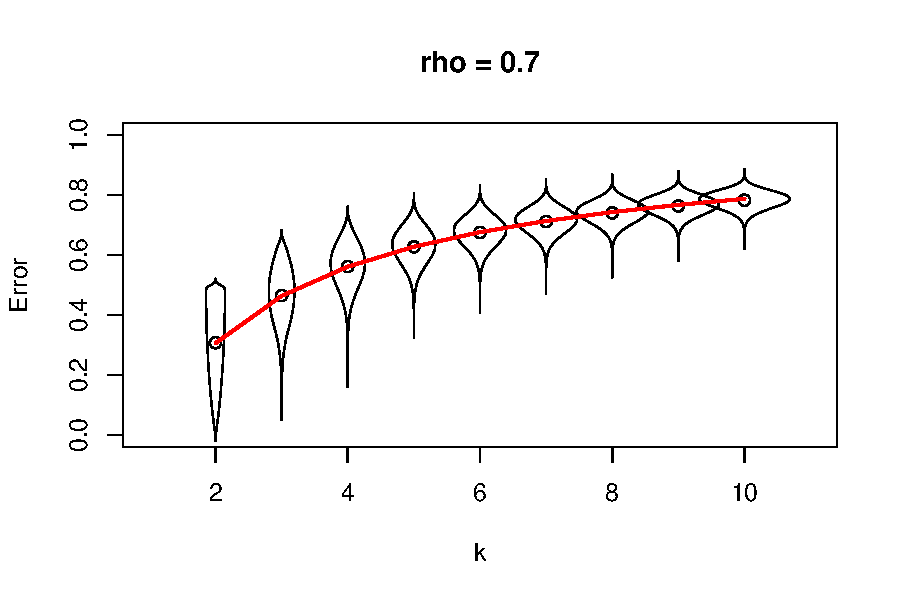
\includegraphics[scale = 0.5]{../extrapolation/illus_err_0_7.pdf}
\end{center}
\end{frame}

\begin{frame}
\frametitle{Defining the $U$-function}
Define $U_x(y)$ as follows:
\begin{itemize}
\item Suppose we have test instance (face) $x$ whose true label (person) is $y$.
\item Let $Y'$ be a random \emph{incorrect} label (person).
\item Use the classifier to guess whether $x$ belongs to $y$ or $Y'$.
\item Define $U_x(y)$ as the probabilility of success (randomizing over training data).
\end{itemize}
\end{frame}

\begin{frame}
\frametitle{Toy example}
\begin{center}
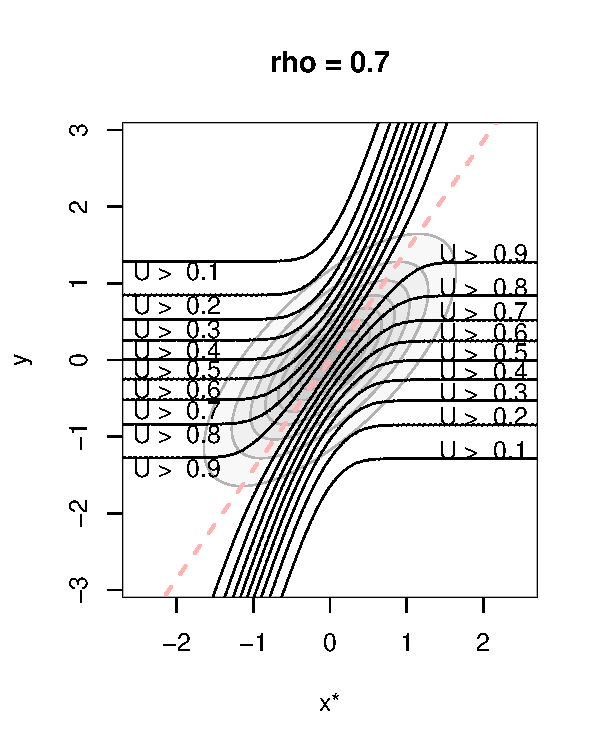
\includegraphics[scale = 0.5]{../extrapolation/illus_ufunc_0_7.pdf}
\end{center}
\[
U_y(x) = \Pr[d(x, \rho Y') > d(x, \rho y)],\text{ for }Y' \sim N(0,1).
\]
\end{frame}

\begin{frame}
\frametitle{Defining $\bar{D}(u)$}
\begin{itemize}
\item Define random variable as $U_Y(X)$ for $(Y, X)$ drawn from the joint distribution.\pause
\item $\bar{D}(u)$ is the cumulative distribution function of $U$,
\[
\bar{D}(u) = \Pr[U_Y(X) \leq u].
\]
\pause
\end{itemize}
\begin{center}
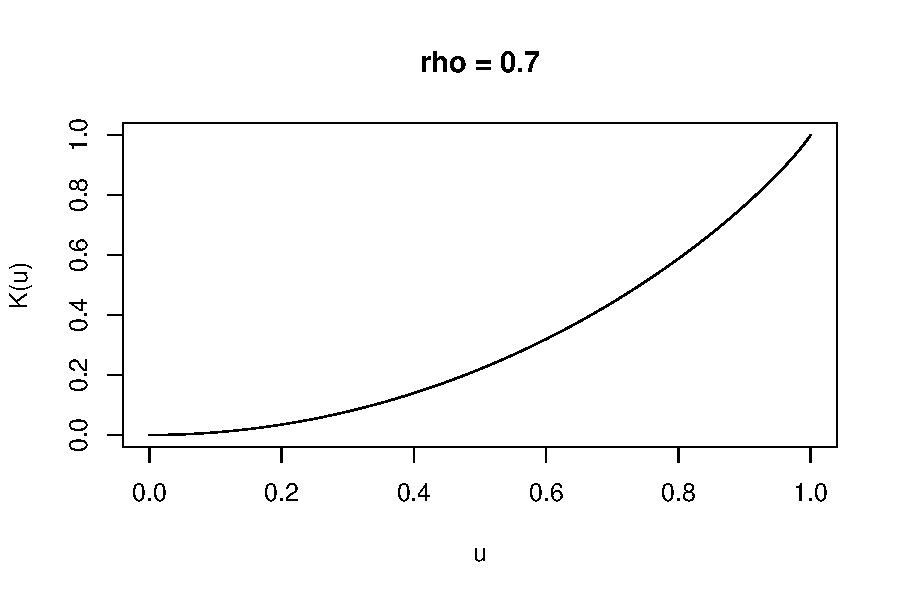
\includegraphics[scale = 0.45]{../extrapolation/illus_kfunc_0_7.pdf}
\end{center}
\end{frame}

\begin{frame}
\frametitle{Computing average risk}
\[
\text{AvRisk}_k = (k-1) \int \bar{D}(u) u^{k-2} du.
\]
\begin{center}
($k$ = 2)
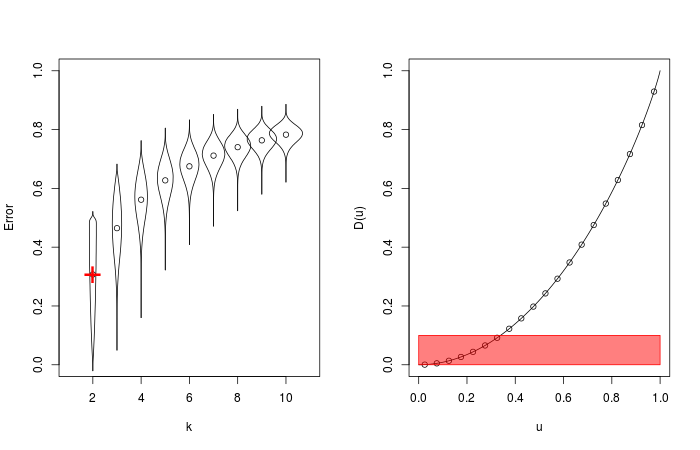
\includegraphics[scale = 0.4, clip=true, trim=0 0.1in 0 0.7in]{../extrapolation/rho_0_7_fmla2.png}
\end{center}
\end{frame}

\begin{frame}
\frametitle{Computing average risk}
\[
\text{AvRisk}_k = (k-1) \int \bar{D}(u) u^{k-2} du.
\]
\begin{center}
($k$ = 3)
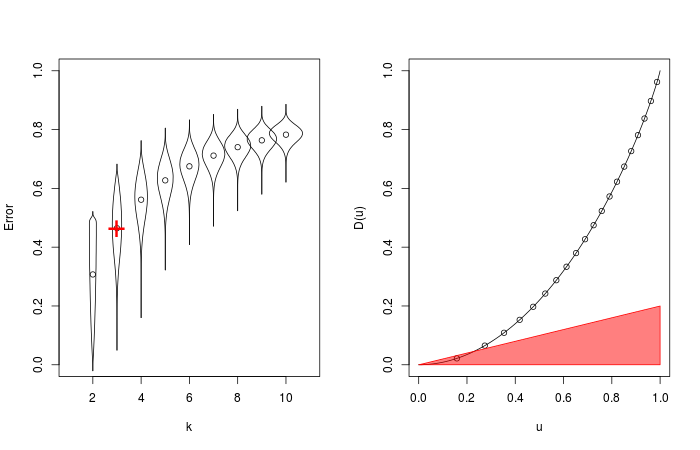
\includegraphics[scale = 0.4, clip=true, trim=0 0.1in 0 0.7in]{../extrapolation/rho_0_7_fmla3.png}
\end{center}
\end{frame}

\begin{frame}
\frametitle{Computing average risk}
\[
\text{AvRisk}_k = (k-1) \int \bar{D}(u) u^{k-2} du.
\]
\begin{center}
($k$ = 4)
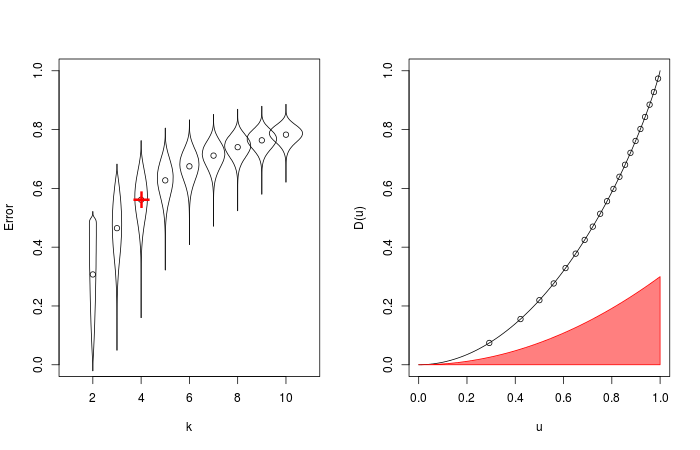
\includegraphics[scale = 0.4, clip=true, trim=0 0.1in 0 0.7in]{../extrapolation/rho_0_7_fmla4.png}
\end{center}
\end{frame}

\begin{frame}
\frametitle{Computing average risk}
\[
\text{AvRisk}_k = (k-1) \int \bar{D}(u) u^{k-2} du.
\]
\begin{center}
($k$ = 5)
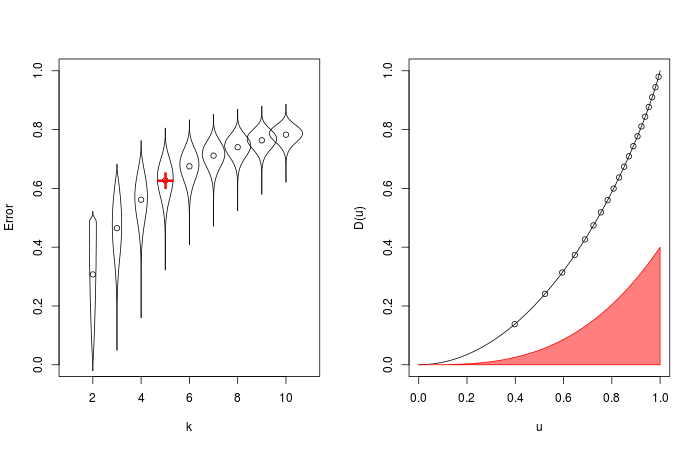
\includegraphics[scale = 0.4, clip=true, trim=0 0.1in 0 0.7in]{../extrapolation/rho_0_7_fmla5.png}
\end{center}
\end{frame}

\begin{frame}
\frametitle{Computing average risk}
\[
\text{AvRisk}_k = (k-1) \int \bar{D}(u) u^{k-2} du.
\]
\begin{center}
($k$ = 6)
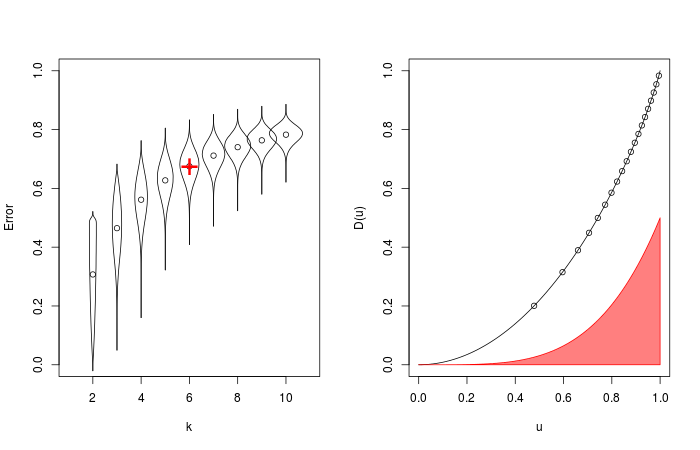
\includegraphics[scale = 0.4, clip=true, trim=0 0.1in 0 0.7in]{../extrapolation/rho_0_7_fmla6.png}
\end{center}
\end{frame}

\begin{frame}
\frametitle{Computing average risk}
\[
\text{AvRisk}_k = (k-1) \int \bar{D}(u) u^{k-2} du.
\]
\begin{center}
($k$ = 7)
\includegraphics[scale = 0.4, clip=true, trim=0 0.1in 0 0.7in]{../extrapolation/rho_0_7_fmla7.png}
\end{center}
\end{frame}

\begin{frame}
\frametitle{Computing average risk}
\[
\text{AvRisk}_k = (k-1) \int \bar{D}(u) u^{k-2} du.
\]
\begin{center}
($k$ = 8)
\includegraphics[scale = 0.4, clip=true, trim=0 0.1in 0 0.7in]{../extrapolation/rho_0_7_fmla8.png}
\end{center}
\end{frame}

\begin{frame}
\frametitle{Computing average risk}
\[
\text{AvRisk}_k = (k-1) \int \bar{D}(u) u^{k-2} du.
\]
\begin{center}
($k$ = 9)
\includegraphics[scale = 0.4, clip=true, trim=0 0.1in 0 0.7in]{../extrapolation/rho_0_7_fmla9.png}
\end{center}
\end{frame}

\begin{frame}
\frametitle{Computing average risk}
\[
\text{AvRisk}_k = (k-1) \int \bar{D}(u) u^{k-2} du.
\]
\begin{center}
($k$ {\tiny =}\hspace{0.025in}10)
\includegraphics[scale = 0.4, clip=true, trim=0 0.1in 0 0.7in]{../extrapolation/rho_0_7_fmla10.png}
\end{center}
\end{frame}

\begin{frame}
\frametitle{Implication: estimate $\bar{D}(u)$ to predict risk}
\begin{itemize}
\item Theoretical result links $k$-class average risk to $\bar{D}(u)$ function
\item In real data, we do not know $\bar{D}(u)$ since it depends on the unknown joint distribution
\item However, given a model, we can estimate $\bar{D}(u)$
\end{itemize}
\end{frame}

\begin{frame}
\frametitle{Subsampled risk estimates}

\begin{columns}
\begin{column}{0.5\textwidth}
\begin{itemize}
\item Suppose we have data for $k$ classes (subsampled from $\pi$)
\item The test error $\text{TestErr}_k$ is an unbiased estimate for $\text{AvRisk}_k$
\item For any $\ell < k$, we can estimate $\text{AvRisk}_\ell$ by \emph{subsampling} the $k$ classes, and taking the average test risk, $\text{AvTestErr}_\ell$.
\end{itemize}
\end{column}
\begin{column}{0.5\textwidth}
\begin{tabular}{|c|c|}
\hline
$k = 4$ & \faceA vs \faceB vs \faceC vs \faceD \\ \hline
$k = 3$ 
 & \faceA vs \faceB vs \faceC \\
 & \faceA vs \faceB vs \faceD \\
 & \faceA vs \faceC vs \faceD \\
 & \faceB vs \faceC vs \faceD \\ \hline
$k = 2$
 & \faceA vs \faceB \\
 & \faceA vs \faceC \\
 & \faceA vs \faceD \\
 & \faceB vs \faceC \\
 & \faceB vs \faceD \\
 & \faceC vs \faceD \\ \hline
\end{tabular}
\end{column}
\end{columns}

\end{frame}

\begin{frame}
\frametitle{Parametric modelling approach}
Assume that for set of basis functions $h_1,\hdots, h_\ell$, we have

\[
\bar{D}(u) = \sum_{\ell = 1}^m \beta_\ell h_\ell(u).
\]

Then
\[
\text{AvRisk}_{k} = \sum_{\ell = 1}^m \beta_\ell H_{\ell,k} = \beta^T \vec{H}_k
\]
where
\[
H_{\ell,k} = (k-2) \int_0^1 h_\ell(u) u^{k-2} du.
\]
and $\vec{H}_k = (H_{1,k},\hdots, H_{\ell, k})$
\end{frame}

\begin{frame}
\frametitle{Prediction extrapolation as regression}
\begin{enumerate}
\item Choose basis $h_1,\hdots, h_\ell$
\[
\bar{D}(u) = \sum_{\ell = 1}^m \beta_\ell h_\ell(u).\pause
\]
\item Obtain subsampled test errors $\text{AvTestErr}_2,\hdots, \text{AvTestErr}_k$.\pause
\item Fit regression model
\[
\hat{\beta} = \argmin_\beta \sum_{i=2}^{k} \left(\text{AvTestErr}_i - \vec{H}_i^T \beta_\ell\right)^2
\]\pause
\item For $K > k$, predict $\text{AvRisk}_K$ as
\[
\widehat{\text{AvRisk}}_K = \vec{H}_K^T \beta_\ell.
\]
\end{enumerate}
\end{frame}

\begin{frame}
\frametitle{Examples of basis functions}
\begin{itemize}
\item Polynomials, $1, x, x^2, \hdots$
\item Cubic splines
\item Linear splines, $[x-t_\ell]_+$
\end{itemize}

Optional constraint: assume $\beta$ is \emph{non-negative}.  In the case of linear splines, this results in a \emph{convex} fit.
\end{frame}

\section{Applications}

\begin{frame}
\sectionpage
\end{frame}

\begin{frame}
\frametitle{Facial recognition example}
\begin{itemize}
\item Data: faces from ``Labeled Faces in the Wild.''
\item 1672 people with at least 2 photos
\item Featurization: trained neural network from OpenFace
\end{itemize}
\begin{center}
\includegraphics[scale = 0.3]{openface_struc.png}
\end{center}
\end{frame}

\begin{frame}
\frametitle{Facial recognition example}
\begin{columns}
\begin{column}{0.5\textwidth}
\begin{itemize}
\item Let us first subsample 400 faces (out of 1672)
\item Randomly choose 1 face as training and 1 as test for each person
\item Use 1-nearest neighbor.
\begin{itemize}
\item NOTE: 1-NN with 1 example/class is equivalent to LDA with $\Sigma = I$: this fits marginal classifier assumption!
\end{itemize}
\end{itemize}
\pause
\end{column}
\begin{column}{0.5\textwidth}
\begin{center}
\includegraphics[scale = 0.4]{../facerec/acc_plot1.pdf}
\end{center}
\pause
\end{column}
\end{columns}
\vspace{0.1in}
\textbf{Can we predict the accuracy on the full set of 1672?}
\end{frame}

\begin{frame}
\frametitle{Estimated $\bar{D}(u)$}
Using linear spline basis ($p=10000$) and nonnegativity constraint. 
\begin{center}
\includegraphics[scale = 0.5]{../facerec/du_est.pdf}
\end{center}
\end{frame}

\begin{frame}
\frametitle{Estimated risk}
Compare to test risk at $K = 1672$
\begin{center}
\includegraphics[scale = 0.4]{../facerec/acc_plot2.pdf}
\end{center}
\end{frame}

\begin{frame}
\frametitle{Estimated risk: more experiments}
\begin{center}
\begin{tabular}{cc}
\includegraphics[scale = 0.2]{../facerec/sub_100.pdf} &
\includegraphics[scale = 0.2]{../facerec/sub_200.pdf} \\
\includegraphics[scale = 0.2]{../facerec/sub_400.pdf} &
\includegraphics[scale = 0.2]{../facerec/sub_800.pdf}
\end{tabular}
\end{center}
\end{frame}

\begin{frame}
\frametitle{Estimated risk: more experiments}
\begin{center}
\includegraphics[scale = 0.6]{../facerec/sub_preds.pdf}
\end{center}
\end{frame}

\begin{frame}
\frametitle{Telugu OCR example}
\begin{center}
\includegraphics[scale = 0.4]{telugu_chars.png}

\includegraphics[scale = 0.3]{telugu_cnn.png}
\end{center}
\end{frame}

\begin{frame}
\frametitle{Telugu OCR example}
\begin{center}
\begin{tabular}{|c||c|c|c|c|c|}\hline
Classifier      & Test $\text{err}^{(20)}$ & Test $\text{err}^{(400)}$ & $\hat{p}^{EXP}_{400}$ & $\hat{p}^{POS}_{400}$ & $\hat{p}^{(5)}_{400}$\\ \hline
Naive Bayes     & 0.049                   & 0.399                   & 0.108              & \textbf{0.142}      & 0.079             \\ \hline
Logistic        & 0.078                   & 0.289                   & 0.166              & \textbf{0.188}      & 0.130             \\ \hline
SVM             & 0.140                   & 0.455                   & 0.299              & \textbf{0.313}      & 0.227             \\ \hline
$\epsilon$-NN   & 0.049                   & 0.409                   & 0.084              & \textbf{0.590}      & 0.102             \\ \hline
Deep neural net & 0.005                   & 0.014                   & \textbf{0.011}     & 0.093               & 0.010             \\ \hline
\end{tabular}

Performance extrapolation: predicting the accuracy on 400 classes using data from 20 classes on a Telugu character dataset.
$\epsilon = 0.002$ for $\epsilon$-nearest neighbors.
\end{center}
\end{frame}

\section*{Acknowledgements}

\begin{frame}
\sectionpage
\end{frame}

\begin{frame}
\begin{center}
\includegraphics[scale = 0.04]{IMG_0703.JPG}

\includegraphics[scale = 0.6]{Taylor_2010.jpg}
\end{center}
\end{frame}

\begin{frame}
\begin{center}
\begin{tabular}{c}
\includegraphics[scale = 0.7]{2014_Efron-indoors.jpg}\\
\includegraphics[scale = 0.16]{poldrack_photo2_400.jpg}\\
\includegraphics[scale = 0.16]{tsachypic.jpg}
\end{tabular}
\end{center}
\end{frame}

\begin{frame}
\begin{center}
\includegraphics[scale = 0.3]{DSCN3964.JPG}
\end{center}
\end{frame}

\section*{The end}

\begin{frame}
\sectionpage
\end{frame}



\end{document}
\end{frame}
\end{document}


